\documentclass[aspectratio=169]{beamer}

\usepackage{cppenv, recdefs}

\usepackage{drawstack}
\usepackage{fourier}
\usepackage{fontspec}
\setmonofont{Ubuntu Mono}

\usetheme{CambridgeUS}

\title{Exception Handling and Exception Safety}
\subtitle{CS100 Lecture 24}
\author{GKxx}
\date{\today}

\AtBeginSubsection{
  \begin{frame}{Contents}
    \tableofcontents[currentsection, currentsubsection]
  \end{frame}
}

\begin{document}

\begin{frame}
  \maketitle
\end{frame}

\begin{frame}{Contents}
  \tableofcontents
\end{frame}

\section{Things tend to go wrong.}

\begin{frame}[fragile]{Input failure}
  \begin{cpp}[\small]
  int num_of_people;
  std::cin >> num_of_people;
  \end{cpp}
  What happens when the input is not an integer?
  \pause
  \begin{cpp}[\small]
  if (!std::cin) {
    // handle input failure
  }
  \end{cpp}
\end{frame}

\begin{frame}[fragile]{\ilcpp{strcpy}}
  You are asked to write a \ilcpp{strcpy} function...
  \begin{cpp}[\small]
void strcpy(char *dest, const char *source) {
  while (*source)
    *dest++ = *source++;
  *dest = '\0';
}
  \end{cpp}
  \pause
  In reality, things may go wrong:
  \begin{itemize}
    \item Null pointers? Or even worse - wild pointers?
    \item Buffer overflow?
  \end{itemize}
\end{frame}

\begin{frame}[fragile]{Which is better?}
  \begin{columns}
    \begin{column}{0.5\textwidth}
      1. Terminate the program on failure and report the error.
      \begin{cpp}
void strcpy(char *dest, const char *source) {
  if (!dest || !source) {
    std::cerr << "strcpy arguments invalid.\n";
    exit(1);
  }
  while (*source)
    *dest++ = *source++;
  *dest = '\0';
}
      \end{cpp}
    \end{column}
    \begin{column}{0.5\textwidth}
      2. Return false on failure:
      \begin{cpp}
bool strcpy(char *dest, const char *source) {
  if (!dest || !source)
    return false;
  while (*source)
    *dest++ = *source++;
  *dest = '\0';
  return true;
}
      \end{cpp}
    \end{column}
  \end{columns}
\end{frame}

\begin{frame}[fragile]{Which is better?}
  \begin{columns}
    \begin{column}{0.5\textwidth}
      3. Be silent to errors.
      \begin{cpp}
void strcpy(char *dest, const char *source) {
  if (dest && source) {
    while (*source)
      *dest++ = *source++;
    *dest = '\0';
  }
}
      \end{cpp}
    \end{column}
    \begin{column}{0.5\textwidth}
      4. Use assertions.
      \begin{cpp}
void strcpy(char *dest, const char *source) {
  assert(dest != NULL);
  assert(source != NULL);
  while (*source)
    *dest++ = *source++;
  *dest = '\0';
}
      \end{cpp}
    \end{column}
  \end{columns}
  A good blog on this topic: \url{https://blog.csdn.net/myan/article/details/1921}
\end{frame}

\section{Exception handling}

\subsection{\ilcpp{throw}}

\begin{frame}[fragile]{Throwing an exception}
  \begin{cpp}[\small]
    class Dynarray {
      std::size_t m_length;
      int *m_storage;
    
    public:
      int &at(std::size_t n) {
        if (n >= m_length)
          throw std::out_of_range{"Dynarray subscript out of range!"};
        return m_storage[n];
      }
    };
  \end{cpp}
\end{frame}

\begin{frame}{Standard exceptions}
  \begin{center}
    \includegraphics[width=0.7\textwidth]{img/ExceptionClasses.jpg}
  \end{center}
  \begin{itemize}
    \item \ilcpp{std::logic_error}, \ilcpp{std::runtime_error} and their subclasses are defined in \ilcpp{<stdexcept>}.
  \end{itemize}
\end{frame}

\begin{frame}{Standard exceptions}
  \begin{itemize}
    \item The normal \ilcpp{new} and \ilcpp{new[]} operators throw \ilcpp{std::bad_alloc} when running out of memory.
    \item \ilcpp{dynamic_cast} for references throws \ilcpp{std::bad_cast} when the cast fails.
    \begin{itemize}
        \item \ilcpp{dynamic_cast} for pointers does not throw. It returns \ilcpp{nullptr} on failure.
    \end{itemize}
    \pause
    \item \ilcpp{std::system_error} is thrown in many cases, especially in functions that interface with \blue{OS facilities}, e.g. the constructor of \ilcpp{std::thread}.
    \item \ilcpp{<chrono>} defines \ilcpp{std::nonexistent_local_time} and \ilcpp{std::ambiguous_local_time} representing some errors related to time settings.
  \end{itemize}
\end{frame}

\begin{frame}[fragile]{Standard exceptions}
  \ilcpp{operator[]} for STL containers does not check boundaries, but \ilcpp{at()} does.
  \begin{cpp}
    std::vector<int> v;
    v.at(0) = 42; // Throws std::out_of_range.
    v[0] = 42;    // Does not throw, but undefined behavior
                  // (and often severe runtime error).
  \end{cpp}
  We will see that exceptions \ilcpp{throw}n could be \ilcpp{catch}ed and handled.
\end{frame}

\begin{frame}[fragile]{Stack unwinding}
  \begin{columns}
    \begin{column}{0.5\textwidth}
      \begin{cpp}[\small]
    void func(int n) {
      std::string s;
      std::cin >> s;
      int *p = new int[n];
      // ...
    }
    int main() {
      int size = 100;
      func(size);
      // ...
    }
      \end{cpp}
    \end{column}
    \begin{column}{0.5\textwidth}
      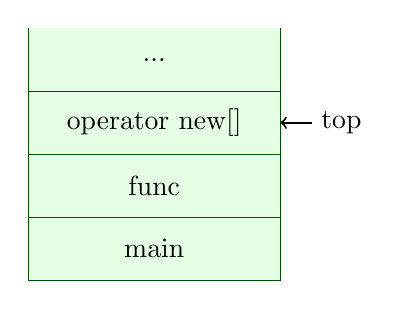
\begin{tikzpicture}[scale=0.8]
        \stacktop{}
        \cell{\ilcpp{operator new[]}}\cellptr{top}
        \cell{\ilcpp{func}}
        \cell{\ilcpp{main}}
      \end{tikzpicture}
    \end{column}
  \end{columns}
  Suppose \ilcpp{operator new[]} encounters shortage of memory...
\end{frame}

\begin{frame}[fragile]{Stack unwinding}
  \begin{columns}
    \begin{column}{0.4\linewidth}
      \begin{cpp}[\small]
@\onslide<4>{\pinkbox}@    void func(int n) {
@\onslide<3>{\pinkbox}@      std::string s;
      std::cin >> s;
@\onslide<1,2>{\pinkbox}\onslide<1>{\danger}@    int *p = new int[n];
      // ...
    }
    int main() {
@\onslide<6>{\pinkbox}@      int size = 100;
@\onslide<5>{\pinkbox}@      func(size);
      // ...
    }
      \end{cpp}
    \end{column}
    \begin{column}{0.6\linewidth}
      \begin{enumerate}
        \onslide<1->\item During the creation of \ilcpp{p}, \ilcpp{std::bad_alloc} is raised in \ilcpp{operator new[]}.
        \onslide<2->\item Control flow returns to \ilcpp{func}.
        \onslide<3->\item \ilcpp{s} is destroyed.
        \onslide<4->\item \ilcpp{n} is destroyed.
        \onslide<5->\item Control flow returns to \ilcpp{main}.
        \onslide<6->\item \ilcpp{size} is destroyed.
      \end{enumerate}
    \end{column}
  \end{columns}
  \onslide<7->
  \begin{notice}
    Stack unwinding is only guaranteed to happen for \textbf{caught} exceptions. If an exception is not caught, whether the stack is unwound is \textbf{implementation-defined}.
  \end{notice}
\end{frame}

\subsection{\ilcpp{try}-\ilcpp{catch}}

\begin{frame}[fragile]{Catch an exception}
  \begin{cpp}
    void func(int n) {
      std::string s;
      std::cin >> s;
      int *p = new int[n];
      // ...
    }
    int main() {
      try {
        int size = 100;
        func(size);
      } catch (const std::bad_alloc &e) {
        // deal with shortage of memory here.
      }
      // ...
    }
  \end{cpp}
  \textit{More Effective C++} Item 13: Catch exceptions by reference.
\end{frame}

\begin{frame}[fragile]{\ilcpp{what()}}
  The error message could be obtained via the `\ilcpp{what}' member function, which is \ilcpp{virtual}, \ilcpp{const} and \ilcpp{noexcept}.
  \begin{cpp}
    void fun() {
      throw std::runtime_error("I love watermelons.");
    }
    int main() {
      try {
        fun();
      } catch (const std::runtime_error &re) {
        std::cout << re.what() << std::endl;
      }
    }
  \end{cpp}
  Output:
  \begin{txt}
    I love watermelons.
  \end{txt}
\end{frame}

\begin{frame}[fragile]{Catch an exception}
  \begin{cpp}
    void f(const std::vector<int> &v) {
      try {
        auto i = 42;
        auto copy = v;
        int x = copy.at(100);
        g(x);
      } catch (const std::bad_alloc &ba) {
        // deal with shortage of memory
      } catch (const std::out_of_range &oor) {
        // deal with illegal subscript '100'
      } catch (...) {
        // What else may happen (probably in 'g(x)')? We are not sure.
        throw; // Throw the exception again.
      }
      std::cout << "returns.\n";
    }
  \end{cpp}
\end{frame}

\newcommand{\commenter}[1]{\footnotesize\gray{#1}}

\begin{frame}[fragile]{Catch an exception}
  \begin{cpp}
    void f(const std::vector<int> &v) {
      try {
@\onslide<3>{\pinkbox}@        auto i = 42;@\onslide<3>{\quad\quad\quad\quad\commenter{`i' is destroyed}}@
@\onslide<2>{\pinkbox}@        auto copy = v;@\onslide<2>{\quad\commenter{`copy' is destroyed}}@
    @\onslide<1>{\pinkbox\danger}@  int x = copy.at(100);@\onslide<1>{\quad\quad\quad\commenter{throws std::out\_of\_range}}@
        g(x);
@\onslide<4>{\pinkbox}@      } catch (const std::bad_alloc &ba) {@\onslide<4>{\quad\commenter{Not matched}}@
        // deal with shortage of memory
@\onslide<5>{\pinkbox}@      } catch (const std::out_of_range &oor) {@\onslide<5>{\quad\commenter{Matched}}@
@\onslide<6>{\pinkbox}@        // deal with illegal subscript '100'
      } catch (...) {
        // What else may happen (probably in 'g(x)')? We are not sure.
        throw; // Throw the exception again.
      }
@\onslide<7>{\pinkbox}@      std::cout << "returns\n";@\onslide<7>{\quad\commenter{Control flow continues here}}@
    }
  \end{cpp}
\end{frame}

\begin{frame}[fragile]{Catch by base class}
  \ilcpp{operator new[]} raises \ilcpp{std::bad_alloc} when out of memory.
  \begin{itemize}
    \item But if the array-new length is obviously invalid, an instance of \ilcpp{std::bad_array_new_length} is raised.
    \begin{cpp}
    new int[-1]; // negative size
    new int[3]{2, 3, 4, 6, 8}; // too many initializers
    new int[LONG_MAX][100]; // too large
    \end{cpp}
    \pause
    \item \ilcpp{catch (const std::bad_alloc &)} also catches it, because of \textbf{inheritance}:
    \begin{figure}[h]
      \centering
      \includegraphics[scale=0.7]{img/bad_array_new_length-inheritance.png}
    \end{figure}
  \end{itemize}
\end{frame}

\begin{frame}[fragile]{Catch by base class}
  \begin{cpp}
    try {
      do_something();
    } catch (const std::runtime_error &re) {
      // deal with runtime_error
    } catch (const std::exception &e) {
      // deal with other kinds of exceptions
    } catch (...) {
      // deal with other things
    }
  \end{cpp}
  \pause
  Note: Other things (e.g. a string) can also be \ilcpp{throw}n.
  \begin{cpp}
    throw "I don\'t want to talk to you.";
    throw 42;
  \end{cpp}
  In this case, these things are caught by \ilcpp{catch (...)}.
\end{frame}

\begin{frame}[fragile]{Catch by base class}
  \bluett{catch} clauses are examined one-by-one.
  \begin{cpp}
    try {
      do_something();
    } catch (const std::exception &e) {
      std::cout << "exception\n";
    } catch (const std::runtime_error &re) {
      std::cout << "runtime_error\n";
    } catch (...) {
      // deal with other things
    }
  \end{cpp}
  If an instance of \ilcpp{std::runtime_error} is thrown, it will be caught by ``\ilcpp{catch (const std::exception \&)}'' instead of ``\ilcpp{catch (const std::runtime_error \&)}'' in this case.
\end{frame}

\begin{frame}[fragile]{Stack unwinding}
  \begin{cpp}[\small]
    void fun() {
@\onslide<3>{\pinkbox}@      int i = 42;@\onslide<3>{\quad\quad\commenter{`i' is destroyed}}@
@\onslide<2>{\pinkbox}@      std::vector<int> v;@\onslide<2>{\quad\commenter{`v' is destroyed}}@
    @\onslide<1>{\pinkbox\danger}@v.at(i) = 10;@\onslide<1>{\quad\quad\commenter{throws std::out\_of\_range}}@
    }
    int main() {
      try {
@\onslide<5>{\pinkbox}@        std::string str("Hello");@\onslide<5>{\quad\commenter{`str' is destroyed}}@
@\onslide<4>{\pinkbox}@        fun();@\onslide<4>{\quad\quad\commenter{Control flow returns here}}@
@\onslide<6>{\pinkbox}@      } catch (...) {}@\onslide<6>{\quad\commenter{The exception is caught.}}@
    }
  \end{cpp}
\end{frame}

\begin{frame}[fragile]{Notes}
  \begin{itemize}
    \item The \ilcpp{try} block and \ilcpp{catch} blocks are independent scopes. Objects declared in the \ilcpp{try} block cannot be used in \ilcpp{catch} blocks.
    \item When an exception occurs, local objects in the \ilcpp{try} block are destroyed before the exception is caught.
    \item Stack unwinding is only guaranteed to happen for \textbf{caught} exceptions.
    \item If an exception is thrown and not caught, `\ilcpp{std::terminate}' will be called to terminate the program. (defined in \ilcpp{<exception>})
  \end{itemize}
\end{frame}

\begin{frame}[fragile]{Function-\ilcpp{try}-block}
  A function-\ilcpp{try}-block is typically useful for a constructor.
  \begin{cpp}
    class Dynarray {
    public:
      Dynarray(std::size_t n)
          try : m_length(n), m_storage(new int[n]{}) {}
      catch (const std::bad_alloc &ba) {
        std::cerr << "No enough memory.\n";
        throw;
      }
    };
  \end{cpp}
  \begin{itemize}
    \item Exceptions raised both in \blue{constructor initializer list} and \blue{function body} can be caught.
    \item Non-static data members cannot be referred to in such \ilcpp{catch} blocks. \red{(Why?)}
    \pause
    \begin{itemize}
      \item An exception thrown in the constructor indicates that the initialization has failed!
      \item Once an exception is thrown, everything initialized in the \ilcpp{try} block are destroyed.
    \end{itemize}
  \end{itemize}
\end{frame}

\section{Exception safety}

\subsection{Exception safety guarantees}

\begin{frame}{Exception safety guarantees}
  Exception-safe functions offer one of three guarantees:
  \begin{itemize}
    \item \textbf{Nothrow guarantee}: Promise never to throw exceptions.
    \item \textbf{Strong guarantee}: Promise that if an exception is thrown, the state of the program is \textbf{unchanged}, as if the function had not been called (``roll back'').
    \item \textbf{Weak guarantee} (basic guarantee): Promise that if an exception is thrown, everything in the program remains in a valid state (though possibly changed).
    \begin{itemize}
      \item No objects or data structures become corrupted.
      \item All class invariants are satisfied. For example, a \ilcpp{Polynomial} should have at least one coefficient (the constant term). In \ilcpp{Dynarray}, \ilcpp{m_length} should represent the length of the memory block that \ilcpp{m_storage} points to.
    \end{itemize}
  \end{itemize}
  \textit{Effective C++} Item 29: Strive for exception-safe code.
\end{frame}

\begin{frame}[fragile]{Exception safety guarantees}
  The level of an exception safety guarantee measures how hard it is to recover from an exception.
  \begin{cpp}
    void foo(std::vector<int> &values) {
      try {
        values = something();
      } catch (const std::bad_alloc &ba) {
        // Can we assume that 'values' is still in a valid state? (weak guarantee)
        // Can we assume that 'values' remains unchanged? (strong guarantee)
      }
    }
  \end{cpp}
\end{frame}

\begin{frame}{Exception safety guarantees}
  \textit{Effective C++} Item 29:
  \begin{quotation}
    A software system is \textbf{either exception-safe or it's not}. There's no such thing as a partially exception-safe system. If a system has \textbf{even a single function} that's not exception-safe, the system as a whole is not exception-safe.

    A function can usually offer a guarantee no stronger than the \textbf{weakest} guarantee of the functions it calls.
  \end{quotation}
\end{frame}

\begin{frame}[fragile]{Which exception safety guarantee?}
  \begin{cpp}
    class Dynarray {
      int *m_storage;
      std::size_t m_length;
    
    public:
      Dynarray &operator=(const Dynarray &other) {
        if (this != &other) {
          delete[] m_storage;
          m_storage = new int[other.m_length]; // May throw std::bad_alloc
          std::copy(other.m_storage, other.m_storage + other.m_length, m_storage);
          m_length = other.m_length;
        }
        return *this;
      }
    };
  \end{cpp}
  \pause
  \textbf{No guarantee at all!} The data pointed to by \ilcpp{m_storage} has already been destroyed before the exception happens.
\end{frame}

\begin{frame}[fragile]{Which exception safety guarantee?}
  \begin{cpp}
    class Dynarray {
    public:
      Dynarray &operator=(const Dynarray &other) {
        auto new_data = new int[other.m_length];
        std::copy(other.m_storage, other.m_storage + other.m_length, new_data);
        delete[] m_storage;
        m_storage = new_data;
        m_length = other.m_length;
        return *this;
      }
    };
  \end{cpp}
  \pause
  \textbf{Strong guarantee.} Nothing has been changed before \ilcpp{new[]} on the first line throws an exception.
\end{frame}

\begin{frame}[fragile]{Which exception safety guarantee?}
  \begin{cpp}
    class Dynarray {
    public:
      Dynarray &operator=(const Dynarray &other) {
        m_length = other.m_length;
        auto new_data = new int[m_length];
        std::copy(other.m_storage, other.m_storage + m_length, new_data);
        delete[] m_storage;
        m_storage = new_data;
        return *this;
      }
    };
  \end{cpp}
  \pause
  \textbf{No guarantee.} \ilcpp{m_length} is changed too early. If \ilcpp{new[]} throws, \ilcpp{m_length} is not equal to the length of the memory block that \ilcpp{m_storage} points to.
\end{frame}

\begin{frame}[fragile]{Which exception safety guarantee?}
  The ``copy-and-swap'' idiom, talked about in previous recitations.
  \begin{cpp}
    class Dynarray {
    public:
      void swap(Dynarray &other) noexcept {
        using std::swap;
        swap(m_length, other.m_length);
        swap(m_storage, other.m_storage);
      }
      Dynarray &operator=(const Dynarray &other) {
        Dynarray(other).swap(*this);
        return *this;
      }
    };
  \end{cpp}
  \pause
  \textbf{Strong guarantee.} The only thing that may throw an exception is \ilcpp{Dynarray(other)} (which allocates memory through \ilcpp{new[]}).
\end{frame}

\subsection{Exception specification}

\begin{frame}[fragile]{\mono{noexcept} vs \mono{throw()}}
  Before C++11, a function may declare in advance \blue{what} exception(s) it may throw.
  \begin{cpp}
void *operator new(std::size_t size) throw(std::bad_alloc); // May throw std::bad_alloc.
  \end{cpp}
  \pause
  To a function that offers nothrow guarantee: \ilcpp{throw()}
  \begin{cpp}
int add(int a, int b) throw() {
  return a + b;
}
  \end{cpp}
\end{frame}

\begin{frame}[fragile]{\mono{noexcept} vs \mono{throw()}}
  People came to realize that it is \textbf{whether the function throws exceptions or not} that really matters.
  \begin{itemize}
    \item In most cases, knowing the specific exception type offers no more help.
    \item In most cases, all we can do is to catch it through \ilcpp{catch(...)}, report it or do some logging, and then throw it again through \ilcpp{throw;}.
  \end{itemize}
  \pause
  Since C++11, declare \ilcpp{noexcept} for non-throwing functions.
  \begin{cpp}
    class Dynarray {
    public:
      void swap(Dynarray &other) noexcept {
        std::swap(m_storage, other.m_storage);
        std::swap(m_length, other.m_length);
      }
    };
  \end{cpp}
  The \mono{throw()} specifiers have been deprecated and removed in modern C++.
\end{frame}

\begin{frame}{\ilcpp{noexcept}}
  The \ilcpp{noexcept} specifier makes it possible for more optimization.
  \begin{itemize}
    \item When an exception is thrown inside a \ilcpp{noexcept} function, whether the stack is unwound is \textit{implementation-defined}.
    \begin{itemize}
      \item Compilers need not keep the runtime stack in an unwindable state.
    \end{itemize}
    \item Certain functions must be \ilcpp{noexcept} so that they can be called by standard library functions.
  \end{itemize}
\end{frame}

\begin{frame}[fragile]{Move operations are often \ilcpp{noexcept}.}
  Recall that \ilcpp{std::vector<T>} will allocate a larger block of memory when the current memory capacity is not enough.
  \begin{cpp}
    template <typename T>
    class vector {
      T *m_storage;
      T *m_end_of_elem, *m_end_of_storage; // Possible implementation.
    public:
      void push_back(const T &x) {
        if (size() == capacity())
          reallocate(capacity() == 0 ? 1 : capacity() * 2);
        construct_object_at(m_end_of_elem, x);
        ++m_end_of_elem;
      }
    private:
      void reallocate(std::size_t new_capacity);
    };
  \end{cpp}
\end{frame}

\begin{frame}[fragile]{Move operations are often \ilcpp{noexcept}.}
  Before C++11, the elements are \textbf{copied} to the new memory block.
  \begin{itemize}
    \item Note: \ilcpp{std::vector<T>} does not use \ilcpp{new[]}, because it needs to separate \textbf{object creation} from \textbf{memory allocation}. The following code uses \ilcpp{allocate_memory}, \ilcpp{construt_object_at} and \ilcpp{destroy_and_deallocate} for demonstration only.
  \end{itemize}
  \begin{cpp}
    template <typename T>
    class vector {
      void reallocate(std::size_t new_capacity) {
        auto new_storage = allocate_memory(new_capacity), p = new_storage;
        for (auto old_data = m_storage; old_data != m_end_of_elem; ++old_data)
          construct_object_at(p++, *old_data);
        destroy_and_deallocate(m_storage);
        m_storage = new_storage;
        m_end_of_elem = p;
        m_end_of_storage = m_storage + new_capacity;
      }
    };
  \end{cpp}
\end{frame}

\begin{frame}[fragile]{Move operations are often \ilcpp{noexcept}.}
  To offer \textbf{strong exception safety guarantee}, \ilcpp{reallocate} needs to ``recall'' the operations once an exception is encountered.
  \begin{cpp}
    template <typename T>
    class vector {
      void reallocate(std::size_t new_capacity) {
        auto new_storage = allocate_memory(new_capacity), p = new_storage;
        @\redtt{try \{}@
          for (auto old_data = m_storage; old_data != m_end_of_elem; ++old_data)
            construct_object_at(p++, *old_data);
        @\redtt{\} catch (...) \{}@
          @\redtt{while (p != new\_storage) destroy(--p);}@
          @\redtt{deallocate(new\_storage); throw;}@
        @\redtt{\}}@
        destroy_and_deallocate(m_storage);
        m_storage = new_storage; m_end_of_elem = p; m_end_of_storage = m_storage + new_capacity;
      }
    };
  \end{cpp}
\end{frame}

\begin{frame}[fragile]{Move operations are often \ilcpp{noexcept}.}
  Since C++11, a reasonable optimization is to \textbf{move} elements, instead of copying them.
  \begin{cpp}
    template <typename T>
    class vector {
      void reallocate(std::size_t new_capacity) {
        auto new_storage = allocate_memory(new_capacity), p = new_storage;
        try {
          for (auto old_data = m_storage; old_data != m_end_of_elem; ++old_data)
            construct_object_at(p++, @\redtt{std::move(*old\_data)}@);
        } catch (...) {
          // Wait ... The elements are moved! How can we recover them?
        }
        // ...
      }
    };
  \end{cpp}
\end{frame}

\begin{frame}[fragile]{Move operations are often \ilcpp{noexcept}.}
  Since C++11, a reasonable optimization is to \textbf{move} elements, instead of copying them.

  Unlike copy, \textbf{move} of an element is a modifying operation.
  \begin{itemize}
    \item The old elements are modified during this procedure.
    \item If a move throws an exception, there is no way of rolling back!
  \end{itemize}

  Due to this consideration, \ilcpp{std::vector<T>} uses the move operation of \ilcpp{T} \textbf{only when it is \ilcpp{noexcept}}.
  \begin{cpp}
    for (auto old_data = m_storage; old_data != m_end_of_elem; ++old_data)
      construct_object_at(p++, @\redtt{std::move\_if\_noexcept(*old\_data)}@);
  \end{cpp}
\end{frame}

\begin{frame}{\ilcpp{noexcept}}
  \ilcpp{noexcept} is only a \textbf{logical guarantee}. A \ilcpp{noexcpet} function may still
  \begin{itemize}
    \item call functions that are not \ilcpp{noexcept}, or
    \item throw exceptions under certain circumstances.
  \end{itemize}
\end{frame}

\begin{frame}{Summary}
  \begin{itemize}
    \item \ilcpp{throw} an exception
    \item \ilcpp{try}-\ilcpp{catch}: catch and handle exceptions
    \item Standard library exceptions: \ilcpp{std::exception}, \ilcpp{std::bad_alloc}, \ilcpp{std::logic_error}, \ilcpp{std::runtime_error}, \ilcpp{std::bad_cast}, ...
    \item Stack unwinding:
    \begin{itemize}
      \item Destroys local objects in reverse order of initialization.
      \item Only guaranteed to happen for \textbf{caught} exceptions.
    \end{itemize}
  \end{itemize}
\end{frame}

\begin{frame}{Summary}
  \begin{itemize}
    \item Exception safety guarantee:
    \begin{itemize}
      \item Nothrow guarantee
      \item Strong guarantee: ``roll back''
      \item Weak guarantee: Promises that everything is in a valid state.
    \end{itemize}
    \item \ilcpp{noexcept}: specifies that a function offers nothrow guarantee.
    \item Move operations are often \ilcpp{noexcept}, because unlike copy, move is a modifying operation.
  \end{itemize}
\end{frame}

\begin{frame}{Homework}
  Make your \ilcpp{Dynarray::operator=} offer the strong exception safety guarantee.
\end{frame}

\end{document}